% Chapter Template

\chapter{Projects/Activities} % Main chapter title
%σύντομη περιγραφή όλων των δραστηριοτήτων που ανέλαβα

\label{Chapter3}

During my internship, I participated in quite a few projects that were mostly related to Beat Hotels product, either bugs resolved or entirely new features created, or Greek Marketing’s requirements. All of these projects will be analyzed in this chapter, expect the ones of Chapter \ref{Chapter4} that will just mentioned so as to avoid repetition.

\section{Project 2: Geo - Npm Package}


\begin{figure}[H]
	\begin{center}
		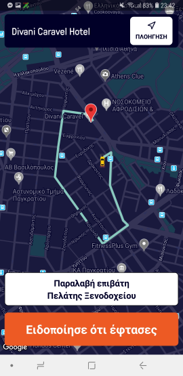
\includegraphics[scale=0.45]{images/my_projects/price_estimator.png}
	\end{center}
	\caption{Approved Pull Request}
\end{figure}

\section{Project 1: Price Estimator- Rides for Approval}

BeatHotel is a totally different product than Beat and a newly introduced one as described in the previous Chapters. For this reason, this new product is combined with a different driver app and a dashboard used by agents, Beat's employees. Agents use the dashboard in order to control rides made through BeatHotel App, start a ride or cancel one if it is needed. This new product does not have any price estimator for the rides made which means that a driver could theoretically add any amount desirable. \par

The project “price estimator” was created for preventing any fraud occurred by drivers. The aim of this project was to estimate the price of a completed ride and compare this price with the actually declared one. In this way, every completed ride is checked  and if it does not pass the validation, it remains as Ride for Approval, so as Agents to check the validate of price gained. \par

This project was the first project ever assigned to me and to one more intern. Our role to this project was to create in Node.js a function for calculating the price of a completed ride based on the data found in database and another function fo validating if the result is approximately equal to the ride's price. We need to mention that every five seconds, each driver sends its location (latitude and longitude), a timestamp (time of the data sent) and other information. So, we used these data gathered in firebase and by using the geo package mentioned earlier and rules of how taxi pricing is in Greece, we managed to get an estimation of the ride. Afterwards, we created one more function for checking the real price with the estimated one. \par

The project lasted about two weeks and it was a great addition to BeatHotel HQ service. We need to clarify that for about a year the service did not have any commissions gained from the driver and that's why it was not a priority at first. Because of this additional feature, Beat's commission is real scenario. \par 

\section{Project 3: Statistics (analyzed in next Chapter)}

"Statistics" project is an external feature in Agent's dashboard that reveals total rides and Gross Merchandise Volume (GMV) gained from BeatHotel service. This project was separated in three main parts, the creation of stats npm package, customized statistics and general statistics, that will be described in detail in next Chapter. Generally, there were added charts in the BeatHotel's web application that present data based on different parameters chosen by Agents. In the chart, the given period's data are also compared with the previous week's or year's data and useful information are extracted for BeatHotel service.

\section{Project 4: Geofence in New Map}
Geofence in New Map- production (feature-deckGLMap)

\section{Project 5: Arc for accepted Drivers in Map}
Arc for accepted Drivers in Map- production (PR)

We want an arc to be added in "Live Map" Tab from the driving vehicle in the map to the pickup location. (12/06/19) (23/05 asana)

\section{Project 6: Babel Configuration for running code in both front-end and back-end}

(13/05/19)

\section{Project 7: Add StartTimestamp- endtimestamp and HQ}
Added to Completed Rides timestamps and link driver to HQ- production (PR)

In "Completed Rides Tab" on Beat Hotels Services - HQ we want to add  the ride ended time named "End Time" in the window which agents see more info about the ride. (6/05/19 asana)

In "Completed Rides Tab" on Beat Hotels Services - HQ we want to add the time of request named "Request Time" of the ride. (requesttimestamp on firebase) in the window which agents see more info about the ride.

In "Completed Rides Tab" on Beat Hotels Services - HQ we want agents by clicking on the Driver's Plates, his profile on HQ ((https://hq-gr.taxibeat.com/driver/edit/9351/) to be appeared.

\section{Project 8: Eliminate Errors in console and eslint errors}
Eliminate Errors in console and eslint errors (PR)

Remove all warnings from console (generated from ESLint) (22/05/19 asana)

\section{Project 9: Add button for unblocking dispatching status-production}
Add button for unblocking dispatching status-production (PR)


\section{Project 10: Landing page for mpaineis-vgaineis (analyzed in next Chapter)}

Landing page for mpaineis-vgaineis is a project referred to the development of a web site for \url{mpaineis-vgaineis.gr} competition of Beat. More specifically, GR Marketing team launched an event in which every week one participant would win a trip abroad. The competition lasted four weeks, and every week there was a different destination. My part to this event was to create the landing page through which every possible user could declare interest in the event, and in this way, to win a trip in one of the destinations. So, I created a responsive to all devices web page, that includes a form for users to declare their interest. The landing page will be online until 7th of June. \par

\section{Project 11: Statistics in Dashboard - "Forecast"}
In Statics in Dashboard Tab, we want in the diagram to be completed for the rest hours of the day that we don't have yet data, from the rides and gmv of the previous week. (18/06)

\section{Project 12: Input location (analyzed in next Chapter)}

BeatHotel is generally a B2B service that aims to fulfill the needs of hotels for a virtual taxi queue. So, the service's dashboards, which is the only way Beat's Agents and Hotels to request for a taxi, used for calling a cub to only one pick-up location, the requested Hotel. However, as the business grows, travel agencies, that were part of the system as well, and some hotels needed to fulfill rides that are having different than Hotel's pick up locations. For this reason, this project occurred and I needed to refactor the Dispatch page, change modal so as to be responsive and add an input for typing any possible different pick-up location. \par

\section{Project 13: Zoom to hotel and driver}

We want when agents are searching for driver plates on "Live Map Tab" to be zoomed in this specific driver. (??)

We want in "Live Map" Tab, to be a filter like "Filter by Plates or Phone" where agents will be able to search a Hotel and the map zooms in the filtered Hotel.

%Θα ήθελα να σας ενημερώσω ότι πλέον μπορείτε στο Live Map, να αναζητήσετε ένα ξενοδοχείο και να κάνει zoom στο αντίστοιχο ξενοδοχείο πάνω στον χάρτη. Να σημειωθεί ότι πρέπει να συμπληρωθεί ακριβώς το ξενοδοχείο που επιθυμείτε εάν πρόκειται για ξενοδοχεία που περιλαμβάνουν την ίδια λέξη. (π.χ. εάν πληκτρολογήσετε την λέξη Divani, δεν θα κάνει zoom σε κάποιο ξενοδοχείο, θα πρέπει να πληκτρολογήσετε Divani Caravel, Divani Apollon, κτλ).

%Zoom in maps: Πλέον στο tab "Live Map", όταν αναζητάτε ένα όχημα βάσει Plates ή Phone, αυτόματα γίνεται zoom, στο οδηγό με αυτά τα στοιχεία. Εδώ να τονιστεί ότι για να γίνει zoom θα πρέπει τα στοιχεία Plates ή Phone να είναι μοναδικά για τον οδηγό εκείνη την στιγμή στον χάρτη. (Εάν δηλαδή μία στιγμή στον χάρτη υπάρχουν δύο οδηγοί που οι πινακίδες τους ξεκινάνε από 13 και πλητρολογήσετε το 13 στο search bar δεν θα γίνει zoom σε κάποιον οδηγό παρά μόνο εάν πληκρολογήσετε ολόκληρη την μοναδική πινακίδα του οδηγού).

\section{Project 14: Restructure Setting Component}

\section{Project 15: Get rid of old maps}

We want to get rid of old maps in completed rides and in approved rides and replace with the new maps. More specifically we have to get rid of the package "React MapboxGL"

%10 pages, 10 projects